\documentclass[14pt,aspectratio=169,xcolor=dvipsnames]{beamer}
\usetheme{SimplePlus}
\usepackage{minted}

\title[short title]{Clase 2: Explorando el PC}
\subtitle{}
\author[NA Barnafi] {Nicolás Alejandro Barnafi Wittwer}
\institute[UC|CMM] 
{
    Pontificia Universidad Católica de Chile \\
    Centro de Modelamiento Matemático
}

\titlegraphic{
    \vspace{-1.8cm}
    \begin{flushright}
      
\includegraphics[height=2.5cm]{../images/logos/puc.png} 
    \end{flushright}
}

\date{07/08/2024}
\setbeamercovered{transparent}

\begin{document}
%%%%%%%%%%%%%%%%%%%%%%%%%%%%%%%%%%%%%%%%%%%%%%%%%%%%%%%
\begin{frame}
    \maketitle
\end{frame}
%%%%%%%%%%%%%%%%%%%%%%%%%%%%%%%%%%%%%%%%%%%%%%%%%%%%%%%
\section{La consola}
%%%%%%%%%%%%%%%%%%%%%%%%%%%%%%%%%%%%%%%%%%%%%%%%%%%%%%%
\begin{frame}\frametitle{Principio}
    \begin{itemize}
        \item La consola (Unix) es una forma de interacción con el PC
        \item Funciona a través de programas
        \item Las interfaces gráficas usan consola
    \end{itemize}
    \begin{flushright}
        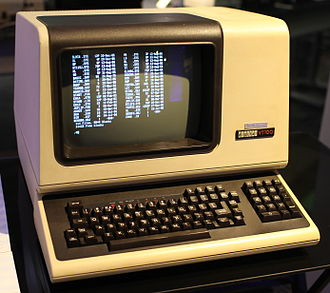
\includegraphics[width=0.4\textwidth]{../images/os-unix.png}
    \end{flushright}
\end{frame}
%%%%%%%%%%%%%%%%%%%%%%%%%%%%%%%%%%%%%%%%%%%%%%%%%%%%%%%
\begin{frame}\frametitle{La consola: Inicio}
La consola Bash en Linux permite interactuar con el PC\footnote{Se puede instalar en Windows con WSL, queda para ayudantía}

    \begin{center}
        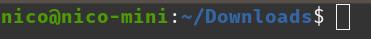
\includegraphics[width=0.6\textwidth]{../images/consola.png}
    \end{center}
\begin{itemize}
    \item \texttt{nico}: Usuario
    \item \texttt{nico-mini}: hostname, nombre de red del PC
    \item \texttt{\~/Downloads}: Carpeta actual
    \item \texttt{\~}: Carpeta 'home'
\end{itemize}
\end{frame}
%%%%%%%%%%%%%%%%%%%%%%%%%%%%%%%%%%%%%%%%%%%%%%%%%%%%%%%
\begin{frame}\frametitle{Sistema de archivos}
En Linux, los archivos funcionan como uno espera:
    \begin{itemize}
        \item Carpeta 1
            \begin{itemize}
                \item Archivo 1
                \item Archivo 2
            \end{itemize}
        \item Carpeta 2
            \begin{itemize}
                \item Carpeta 3
                \item Archivo 3
            \end{itemize}
        \item $\vdots$
    \end{itemize}

\end{frame}
%%%%%%%%%%%%%%%%%%%%%%%%%%%%%%%%%%%%%%%%%%%%%%%%%%%%%%%
\begin{frame}\frametitle{Navegación básica en Bash}
    \begin{itemize}
        \item \texttt{ls}: Mostrar contenido de carpeta
        \item \texttt{cd}: Cambiar de directorio
        \item \texttt{mkdir}: Crear carpeta
        \item \texttt{rm}: Eliminar archivo o carpeta
        \item \texttt{cp}: Copiar archivo o carpeta
        \item \texttt{nano}: Editor de texto
        \item \texttt{cat}: Mostrar archivo
    \end{itemize}

\vspace{1cm} 
Pro-tip: Autocompletar con \texttt{tab}
\end{frame}
%%%%%%%%%%%%%%%%%%%%%%%%%%%%%%%%%%%%%%%%%%%%%%%%%%%%%%%
\begin{frame}[fragile]\frametitle{Concepto de programa}
Ver contenidos de 'Documents':

    $$ \texttt{\$ }\underbrace{\texttt{ls}}_\text{Comando}  \underbrace{Documents}_\text{Argumento} $$
\end{frame}
%%%%%%%%%%%%%%%%%%%%%%%%%%%%%%%%%%%%%%%%%%%%%%%%%%%%%%%
\begin{frame}\frametitle{Argumentos y opciones}
    
    $$ \texttt{\$ }\underbrace{\texttt{ls}}_\text{Comando} \quad \underbrace{\texttt{-l -a --color}}_\text{Opciones} \quad \underbrace{Documents}_\text{Argumento} $$

La más útil: \texttt{--help/-h}. 

\vspace{1cm}
\idea{Veamos...}
\end{frame}
%%%%%%%%%%%%%%%%%%%%%%%%%%%%%%%%%%%%%%%%%%%%%%%%%%%%%%%
\begin{frame}\frametitle{Recap}
    \begin{itemize}
        \item Podemos interactuar con el PC a través de la consola
        \item Linux se ordena con un sistema común de archivos
        \item Las carpetas se pueden navegar y manipular con programas especializados
        \item Los programas pueden aceptar opciones y/o argumentos
        \item En caso de dudas, \texttt{--help/-h}
    \end{itemize}
\end{frame}
%%%%%%%%%%%%%%%%%%%%%%%%%%%%%%%%%%%%%%%%%%%%%%%%%%%%%%%
\begin{frame}
    \maketitle
\end{frame}
\end{document}
